\section{Problemi con giochi cooperativi}

\subsection{Il problema dell'esponenzialità}

Come abbiamo visto, possiamo rappresentare con:
\begin{itemize}
    \item $G = (N,v)$ un gioco, con N giocatori e v una funzione di valore
    \item $v: 2^N \rightarrow \mathbb{R}$ una funzione di valore
\end{itemize}

E abbiamo definito il core come:
\begin{itemize}
    \item x(N) = v(N)
    \item x(s) $\geq$ v(s) $\forall S \subseteq N$
    \item x $\in \mathbb{R}^N$
\end{itemize}

Ma se dovessimo calcolarci la funzione di valore $v$, dovremmo calcolarci tutte
le possibili combinazioni che sono:
\begin{itemize}
    \item \{\}
    \item \{1\}, \{2\}, \{3\} $\dots$ \{n\}
    \item \{1,2\}, \{1,3\}, \{1,4\} $\dots$ \{1,n\}, $\dots$ \{n,n\}
    \item \dots
\end{itemize}

Vediamo che questo valore è \textbf{esponenziale}: $2^N$. Questo è molto chiaro
che funzioni solo da un punto di vista toerico. Nella realtà, gestire problemi
di tipo esponenziale non è chiaramente facile e c'è bisogno di alcune soluzioni
diverse. Le deiniamo \textbf{soluzioni compatte.}

\subsection{Le soluzioni compatte}

Le \textbf{soluzioni compatte} ci permettono di definire il problema in modo
più compatto, in modo da poterlo risolvere in modo più efficiente e
posssibilmente lineare.

\subsubsection{Giochi sui grafi}

Diciamo innanzitutto che i giochi sui grafi sono \textbf{un sotto insieme} dei
giochi cooperativi. Immaginiamo di avere questo grafo:

\begin{figure}[H]
    \begin{center}
        % BEGIN: 8d4x7b5f9j3p
        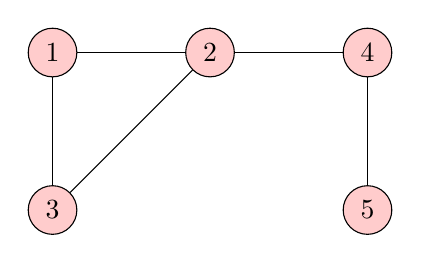
\begin{tikzpicture}
            \node[circle,draw, fill=red!20] (1) at (0,0) {1};
            \node[circle,draw, fill=red!20] (2) at (2,0) {2};
            \node[circle,draw, fill=red!20] (3) at (0,-2) {3};
            \node[circle,draw, fill=red!20] (4) at (4,0) {4};
            \node[circle,draw, fill=red!20] (5) at (4,-2) {5};

            \draw (1) -- (2);
            \draw (1) -- (3);
            \draw (2) -- (4);
            \draw (4) -- (5);
            \draw (3) -- (2);
        \end{tikzpicture}
    \end{center}
\end{figure}
% END: 8d4x7b5f9j3p
La grandezza di questa struttura è al massimo $|N|^2$.

Il problema è che i giochi a grafo \textbf{non sono completi}.

Supponiamo di avere questi valori:
\begin{itemize}
    \item 1,3 = 10
    \item 1,2 = 20
    \item 2,3 = 30
    \item 1,2,3 = 60
\end{itemize}

Con un grafo cosi:
%grao 1,2,3 tutti collegati tra loro con 1,2 peso 20, 1,3 peso 10, 2,3 peso 30
\begin{figure}[H]
    \begin{center}
        % BEGIN: 8d4x7b5f9j3p
        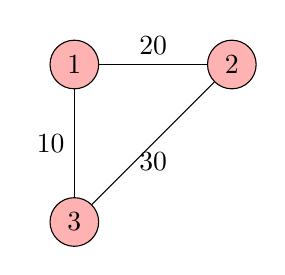
\begin{tikzpicture}
            \node[circle,draw, fill=red!30] (1) at (0,0) {1};
            \node[circle,draw, fill=red!30] (2) at (2,0) {2};
            \node[circle,draw, fill=red!30] (3) at (0,-2) {3};

            \draw (1) -- (2) node [midway, above] {20};
            \draw (1) -- (3) node [midway, left] {10};
            \draw (2) -- (3) node [midway, below] {30};
        \end{tikzpicture}
    \end{center}
\end{figure}
Forse ho capito. Se prendiamo un punto nell'insieme dei giochi cooperativi con v(\{1,2,3\}) = -50, allora nel grafo sopra non esiste e quindi non possono
rappresentare tutte quante le possibili combinazioni. Quindi non sono completi.

\subsubsection{Giochi con contribuzione marginale}

I giochi con contribuzione marginale sono un sottoinsieme dei giochi sui grafi.

Ogni gioco sui grafi può essere rappresentato dai giochi a contribuzione
marginale.

In questo gioco, il valore di una coalizione è dato dalla somma del valore di
tutte le regole che si applicano ad una data coalizione.

Se non stai capendo, sotto c'è la lezione di laboratorio che si collega al
capitolo \ref{MCnets}.

Ad esempio:
\[
    1 \land 2 \rightarrow 20
\]

E possiamo rappresentarlo come:
\begin{figure}[H]
    \begin{center}
        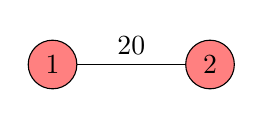
\begin{tikzpicture}
            \node[circle,draw, fill=red!50] (1) at (0,0) {1};
            \node[circle,draw, fill=red!50] (2) at (2,0) {2};

            \draw (1) -- (2) node [midway, above] {20};
        \end{tikzpicture}
    \end{center}
\end{figure}

E se avessimo:
\begin{itemize}
    \item  $1 \land 2 \rightarrow 20$
    \item $1 \land 3 \rightarrow 10$
    \item $2 \land 3 \rightarrow 30$
\end{itemize}

Allora se volessimo rappresentare v(\{1,2,3\}) = -50, dovremmo fare:
\begin{itemize}
    \item $1 \land 2 \land 3 \rightarrow -60 - 50$
\end{itemize}

E allora avremmo:
\[
    v(\{1,2,3\}) = 20 +10 +30 -60 -50 = -50
\]

E tra l'altro i giochi con contribuzione marginale \textbf{corrispondono
    esattamente} coi giochi cooperativi.

%disegna un grafico ovale di un insieme con scritto giochi cooperativi, con dentro un sotto insieme di giohcic oi grafi e un sotto insieme di giochi a coso marginale
\begin{figure}[H]
    \begin{center}
        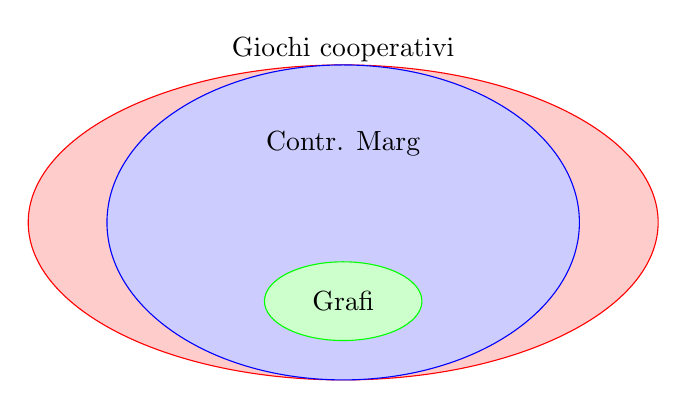
\begin{tikzpicture}
            %disegna un ovale
            \draw [red, fill=red!20] (0,0) ellipse (4cm and 2cm);
            \node at (0,2.2) {Giochi cooperativi};

            %disegna un ovale
            \draw [blue, fill=blue!20] (0,0) ellipse (3cm and 2cm);
            \node at (0,1) {Contr. Marg};

            %disegna un ovale
            \draw [green, fill=green!20] (0,-1) ellipse (1cm and 0.5cm);
            \node at (0,-1) {Grafi};

        \end{tikzpicture}
    \end{center}
\end{figure}

\subsection{Giochi di allocazione}
\label{Giochi di allocazione}

Immaginiamo di avere \textit{2 bambini} che hanno \textit{n giocattoli}. Ogni
giocattolo ha un valore.

\textbf{VA RECUPERATA ROBA DALLE SLIDES DOPO NON HO CAPITO}

Dato il gioco:

\[ G = (N,v), v:2^N \rightarrow R\]
C'è un problema di allocazione.

Per ogni coalizione C, il valore associato è dato dal valore della migliore
coalizione focussandoci sui player solamente in C. Va calcolato il
\textbf{matching massimo} in grafico. La cosa importante è che può essere fatto
in \textbf{tempo polinomiale}.

Cerchiamo di capire cosa vogliamo fare: Siamo in uno \textbf{scenario di
    condivisione}. L'algoritmo considera il migliore modo di costruire le
coalizioni per capire lo scenario migliore di come dividere i beni che ci sono
in gioco.

\subsection{Giochi a voto pesato}

Siamo in questa situazione:
\begin{itemize}
    \item $n$ partiti nel parlamento
    \item Il partito $i$ ha $w_i$ rappresentanti
    \item Una coalizione di partiti può formare un governo solamente se la grandezza è
          almeno $q$
          \begin{itemize}
              \item Solitamente $q \geq | \sum_{i=1}^n w_i|/2$; maggioranza stretta
          \end{itemize}
    \item La notazione è $w(C) = \sum_{i \in c} w_i$
\end{itemize}

Questo può essere descritto come un gioco $G (N,v)$ dove:
\begin{itemize}
    \item N = \{1,2,3, $\dots$, n\}
    \item v(C) = 1 se $w(C) \geq q$, 0 altrimenti
\end{itemize}

\begin{esempio}
\end{esempio}

\begin{itemize}
    \item 1 = 10
    \item 2 = 20
    \item 3 = 5
    \item 4 = 5
\end{itemize}

Ora, vediamo il valore delle coalizioni:
\begin{itemize}
    \item v(\{2,3\}) = 1
    \item v(\{1,2,3\}) = 1
    \item v(\{1,2,3,4\}) = 1
    \item v(\{3,4\}) = 0
\end{itemize}

Anche questi giochi \textbf{non sono completi}, ma diciamo che sono
\textbf{funzionali specificatamente} per alcuni scenari particolari.

\begin{figure}[H]
    \begin{center}
        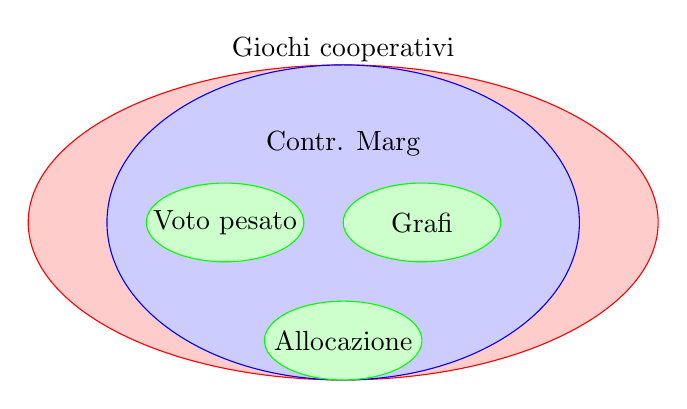
\begin{tikzpicture}
            % Disegna un ovale rosso per "Giochi cooperativi"
            \draw[red, fill=red!20] (0,0) ellipse (4cm and 2cm);
            \node at (0,2.2) {Giochi cooperativi};

            % Disegna un ovale blu per "Contr. Marg"
            \draw[blue, fill=blue!20] (0,0) ellipse (3cm and 2cm);
            \node at (0,1) {Contr. Marg};

            % Disegna un ovale verde per "Grafi"
            \draw[green, fill=green!20] (1,0) ellipse (1cm and 0.5cm);
            \node at (1,0) {Grafi};

            % Disegna un ovale verde per "Allocazione"
            \draw[green, fill=green!20] (0,-1.5) ellipse (1cm and 0.5cm);
            \node at (0,-1.5) {Allocazione};

            % Disegna un ovale verde per "Voto pesato"
            \draw[green, fill=green!20] (-1.5,0) ellipse (1cm and 0.5cm);
            \node at (-1.5,0) {Voto pesato};
        \end{tikzpicture}
    \end{center}
\end{figure}

\begin{domanda}(Puoi calcolare in modo efficiente lo shapley value?)
\end{domanda}

La risposta è che \textbf{dipende}. In alcuni casi, lo shapley value può essere
rappresentato in modo efficiente.

Ma se in alcuni casi la risposta è \textbf{NO}, allora dobbiamo
\textbf{provare} che queste soluzioni sono \textbf{intrattabili.}

\newpage

\section{Classi di compplessità dei problemi}

Definiamo \textbf{problemi facili} i problemi che sono nella classe di
complessità \textbf{polinomiale: P}

\[
    \Sigma_o^P  = P = \prod_o^P
\]

\subsection{Problemi in NP}

NP è la classe di complessità \textbf{non deterministic polinomial: NP}. Il
primo problema è:
\begin{definition}(Il problema dei team)
    Vogliamo fare 2 squadre. L'obiettivo è costruire dei team \textbf{bilanciati}
\end{definition}

\begin{esempio}
    \begin{itemize}
        \item Giocatore 1 = 3
        \item Giocatore 2 = 9
        \item Giocatore 3 = 1
        \item Giocatore 4 = 7
    \end{itemize}

    Il team bilanciato è:
    \begin{itemize}
        \item Team 1 = 1 + 9 = 10
        \item Team 2 = 3 + 7 = 10

    \end{itemize}
\end{esempio}

\textbf{Una prima intuizione:} Vogliamo controllare una soluzione in un tempo ragionevole. Una macchina di turing non
deterministica ha il potere di \textbf{guessare} una soluzione possibile.

\subsection{Problemi in CO-NP}

Con CO-NP classifichiamo i problemi tali che il loro \textbf{complemento} sia
risolvibile in tempo polinomiale usando una macchina di turing non
deterministica. Un problema prototipico: \textit{controllare che una formula
    booleana non è soddisfacibile}.

\subsection{La classe $\Sigma_2^P$}
Questa è la classe di complessità che contiene i problemi che possono essere
risolti in tempo polinomiale da una macchina di turing non deterministica, che
usa una macchina di turing non deterministica come un oracolo a costo unitario.
Un esempio è \textit{decidere se una $\forall\exists$ formula è \textbf{non
        soddisfacibile}}

\subsection{Oltre la gerarchia}
Consideriamo $\#P$ la classe di tutte le funzioni che possono essere calcoalte
da una \textbf{counting turing machine} in tempo polinomiale. Questa
\textbf{counting turing machine} è una macchina di turing non deterministica
che ha un device di output che stampa in binario il numero di computazioni
accettabili indotte dall'input.

Un esempio è \textit{contrare il numero di assegnamenti di verità che
    soddisfano una formula booleana}.

PAGINA 121 DA COPIARE

\begin{table}[H]
    \begin{center}
        \begin{tabular}{|c|c|}
            \hline \textbf{Problema} & \textbf{Classe di complessità} \\
            \hline \
            CORE & coNP-Complete
            \\
            \hline \
            BARGAINING SET & $\prod_2^P$-Complete
            \\
            \hline \
            NUCLEOLUS & $\Delta_2^P$-Complete
            \\
            \hline \
            SHAPLEY VALUE & $\#P$-Complete \\
            \hline
        \end{tabular}
    \end{center}
\end{table}

\subsection{Core e Hardness}

Prendiamo un esempio di grafo:
%1,2,3,4,5 nodi, archi 1,2 peso 4, 1,3 peso 6, 2,3 peso 3, 3,4 peso -4, 2,4 peso -4, 4,5 peso 5
\begin{figure}[H]
    \begin{center}
        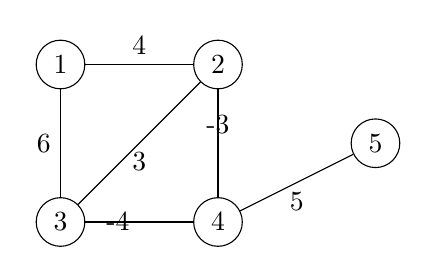
\begin{tikzpicture}
            \node[circle,draw] (1) at (0,0) {1};
            \node[circle,draw] (2) at (2,0) {2};
            \node[circle,draw] (3) at (0,-2) {3};
            \node[circle,draw] (4) at (2,-2) {4};
            \node[circle,draw] (5) at (4,-1) {5};

            \draw (1) -- (2) node [midway, above] {4};
            \draw (1) -- (3) node [midway, left] {6};
            \draw (2) -- (3) node [midway, below] {3};
            \draw (3) -- (4) node [midway, left] {-4};
            \draw (2) -- (4) node [midway, above] {-3};
            \draw (4) -- (5) node [midway, below] {5};
        \end{tikzpicture}
    \end{center}
\end{figure}

Ci chiediamo, \textbf{$C(G) = \emptyset$}? Per rispondere a questa domanda,
definiamo il core:
\begin{itemize}
    \item x(n) = v(n)
    \item $x(S) \geq v(S), S \subseteq N$
\end{itemize}
Assumiamo che esista un taglio nel grafo, e assumiamo che per contraddizione c'è un punto che è all'interno del core.
x(n) = v(n).

Il taglio divide il grafo in $S$ e $T$.

\[
    V(S \cup T) = v(S) + v(T) + valoreDelTaglio
\]

\textbf{Nota:} Gli agenti vogliono splittare se e solo se  \textit{valoreDelTaglio}$<$0

Quindi, la risposta è; \textbf{il core è vuoto se e solo se esiste un taglio
    negativo}

La dimostrazione, parlando chiaramente, \textbf{non l'ho capita lol}.

Controllare che esiste un taglio negativo è un problema \textbf{NP-HARD}. Il
problema complementare è un \textbf{coNP-HARD}

\textbf{Nota:} Massimizzare il taglio è facile, massimo flusso minimo taglio, minimizzare il taglio è difficile.

\subsection{Nucleolus e Hardness}

Ricordiamo un attimo la definizione del Nucleolus:

\begin{definition}(Nucleolus)
    \[
        \mathcal{N}(G) = \{x \in X(G) | \nexists y \in X(G) \ t.c \ \theta(y) \curlyeqprec \theta(x)\}
    \]
\end{definition}

Prendiamo una formula $\varphi = (x_1 \lor x_2) \land x_3 \lor x_4$. Abbiamo un
ordine di indici \{1,2,3,$\dots$,n\}

Assumiamo che le variabili siano \textit{in ordine lessicografico}, quindi in
base al loro indice: $x_1$ è quella meno significativa.

\textbf{Obiettivo:} Trovare l'assegnamento di verità massimo lessicograficamente.

\textit{Esempio:}

\begin{itemize}
    \item $x_2, x_3$ = OK
    \item $x_1, x_4$ = NO
    \item $x_1, x_3$ = OK
\end{itemize}

In questo caso, quello che massimizza è $x_2, x_3$ perché, con pareggio per
$x_3$, abbiamo $x_2$ che ha un valore maggiore rispetto a $x_1$.

\textbf{Strategia:} Partire dalla fine, quindi da quelli più significativi, e controllare \textbf{se esiste un assegnamento di verità} con quella variabile. Se esiste, sicuramente sarà tra i migliori essendo quella più significativa. Questo iterativamente fino al primo (sono polinomiali in numero). Dopo averlo controllato,
esiste un assegnamento di verità per le variabili che soddisfa la formula?

Questo problema è \textbf{$\Delta^P_2$}

\subsection{Nucleolus e Membership}

Definiamo un \textbf{problema lineare}:

\begin{itemize}
    \item $\min_\epsilon$
          \begin{itemize}
              \item e(S,x) $\leq \epsilon_1$
              \item x $\in X(G)$
          \end{itemize}
\end{itemize}

\[
    \forall S \subset N, S \notin W_0 = \{\emptyset\}
\]

Non ho capito un cazzo onestamente e dalle slides non lo capisco. Vedremo come
fare, dai..

\section{Giochi con interazione ristretta}

Pensiamo ad un problema di grafi ma con dei vincoli che non permettono delle
coalizioni tra giocatori.

%Grafico di un alber
\begin{figure}[H]
    \begin{center}
        %Grafico di un albero
        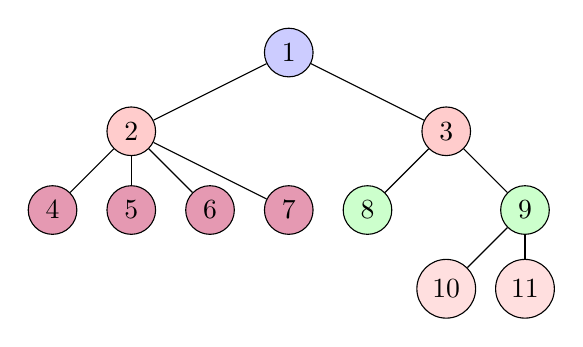
\begin{tikzpicture}
            %nodo centrato 
            \node[circle,draw, fill=blue!20] (1) at (0,0) {1};

            %due nodi 2 e 3 uno a sinistra uno a destra come figli 
            \node[circle,draw, fill=red!20] (2) at (-2,-1) {2};
            \node[circle,draw, fill=red!20] (3) at (2,-1) {3};

            %4 5 6 7 figli di 2
            \node[circle,draw, fill=purple!40] (4) at (-3,-2) {4};
            \node[circle,draw, fill=purple!40] (5) at (-2,-2) {5};
            \node[circle,draw, fill=purple!40] (6) at (-1,-2) {6};
            \node[circle,draw, fill=purple!40] (7) at (0,-2) {7};

            %8 e 9 figli di 3
            \node[circle,draw, fill=green!20] (8) at (1,-2) {8};
            \node[circle,draw, fill=green!20] (9) at (3,-2) {9};

            %10 e 11 figli di 9
            \node[circle,draw, fill=pink!50] (10) at (2,-3) {10};
            \node[circle,draw, fill=pink!50] (11) at (3,-3) {11};

            %Archi 
            \draw (1) -- (2);
            \draw (1) -- (3);
            \draw (2) -- (4);
            \draw (2) -- (5);
            \draw (2) -- (6);
            \draw (2) -- (7);
            \draw (3) -- (8);
            \draw (3) -- (9);
            \draw (9) -- (10);
            \draw (9) -- (11);

        \end{tikzpicture}
    \end{center}
    \caption{Esempio di albero}
\end{figure}

Pensiamola cosi. Gli agenti sono ordinati su una linea.

%disegna una linea con 6 punti chiamati x_1, --- x_6
\begin{figure}[H]
    \begin{center}

        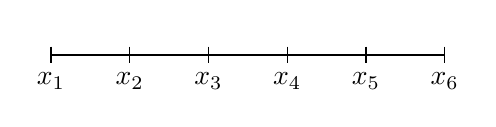
\begin{tikzpicture}
            \draw (0,0) -- (5,0);
            \foreach \x in {0,1,2,3,4,5}
            \draw (\x cm,3pt) -- (\x cm,-3pt);
            \draw (0,0) node[below=3pt] {$x_1$} node[above=3pt] {};
            \draw (1,0) node[below=3pt] {$x_2$} node[above=3pt] {};
            \draw (2,0) node[below=3pt] {$x_3$} node[above=3pt] {};
            \draw (3,0) node[below=3pt] {$x_4$} node[above=3pt] {};
            \draw (4,0) node[below=3pt] {$x_5$} node[above=3pt] {};
            \draw (5,0) node[below=3pt] {$x_6$} node[above=3pt] {};
        \end{tikzpicture}

    \end{center}
    \caption{Esempio di linea}
\end{figure}
Il numero di coalizioni massimo che possiamo formare è \textbf{polinomiale} $\mathcal{O}(n^2)$.

E se invece di una linea avessimo un \textbf{ciclo?}

\begin{figure}[H]
    \begin{center}

        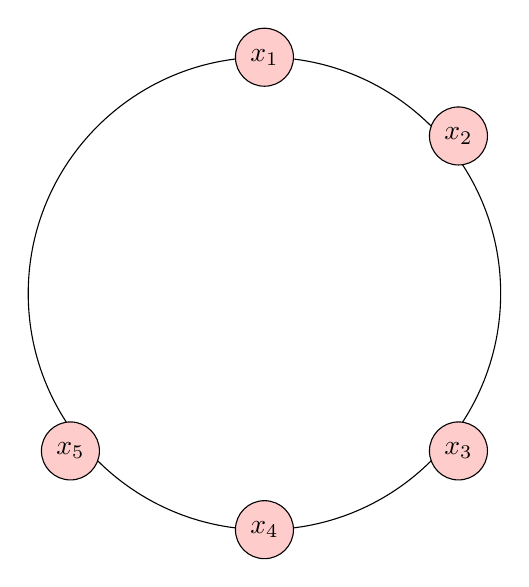
\begin{tikzpicture}
            %disegna un cerchio 
            \draw (0,0) circle (3cm);

            %disegna sul cerchio x1 a x5
            \node[circle,fill=red!20,draw] (1) at (0,3) {$x_1$};
            \node[circle,fill=red!20,draw] (2) at (2.464,2) {$x_2$};
            \node[circle,fill=red!20,draw] (3) at (2.464,-2) {$x_3$};
            \node[circle,fill=red!20,draw] (4) at (0,-3) {$x_4$};
            \node[circle,fill=red!20,draw] (5) at (-2.464,-2) {$x_5$};
        \end{tikzpicture}

    \end{center}
    \caption{Esempio di ciclo}
\end{figure}

Dobbiamo contare il numero di coalizioni. Se cancelliamo l'arco $x_1 x_5$,
diventa una linea. Questo porta ad una linea, allora ancora $\mathcal{O}(n^2)$.

La \textbf{risposta} è: $\mathcal{O}(n^3)$ dato da: $n * n^2$.

E se invece avessimo \textbf{gli alberi}?

A quanto pare sugli alberi il risultato è \textbf{esponenziale}.

\begin{figure}[H]
    \begin{center}
        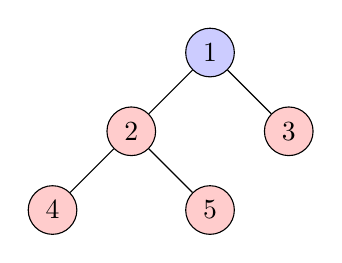
\begin{tikzpicture}
            %disegna un albero con 1 nodo radice e 5 nodi foglia
            \node[circle,fill=blue!20, draw] (1) at (0,0) {1};
            \node[circle,fill=red!20 ,draw] (2) at (-1,-1) {2};
            \node[circle,fill=red!20 ,draw] (3) at (1,-1) {3};
            \node[circle,fill=red!20 ,draw] (4) at (-2,-2) {4};
            \node[circle,fill=red!20 ,draw] (5) at (0,-2) {5};

            \draw (1) -- (2);
            \draw (1) -- (3);
            \draw (2) -- (4);
            \draw (2) -- (5);

        \end{tikzpicture}
    \end{center}
\end{figure}

\newpage